\chapter{实验与分析}
\section{Evaluation}
\label{sec:evaluation}
\subsection{Research Questions}
本章中,我们将围绕以下几个研究问题来展开讨论。
\begin{itemize}
\item {\bf 研究问题1: 宏调用保留。} 针对我们提出的双向预编译器性质2,
  我们的系统希望尽可能地保留宏调用。我们在实验中想知道在实际应用场景中,
  我们的方法能保留多少宏?和其他方法比较,我们的方法是否更优?
\item {\bf 研究问题2: 正确性。} 前文中我们已经证明过,我们提出的双向
  算法满足性质4与性质5。我们在实验中想知道保证这样的正确性在实际应用中
  究竟有多重要?我的方法相比较于那些没有保证正确性的方法,是否在实际
  场景中更优?
\item {\bf 研究问题3: 报错功能。}  在之前的章节中提到,
  当我们的方法发现没有正确的映射方法时,系统将会报错。在实验中我们想知道
  现实中这种情况发生频率多少?会不会存在误报的情况(存在一种可以正确
  映射的方法,但我们的系统没有找到)?
\end{itemize}

为了回答以上几个研究问题,我们在一组生成的Linux内核源代码上做了一组控制
实验。
另外,我们将我们的算法和前文\secref{sec:naive}中提到的两个简答的方法
进行比较。
本章的余下部分,我们会介绍实现与实验的细节。

\subsection{环境搭建}

\subsubsection{JCPP}
我们基于一个开源的C预处理器,JCPP\footnote{\url{http://www.anarres.org/projects/jcpp/}}
实现了我们的双向预处理器,BXCPP。
JCPP是一个完整的,兼容性的,独立的,纯Java实现的C预处理器。
他也可以处理 Apple Objective C 库。

JCPP项目中内置了基本的依照GCC规则的C处理器,
其中定义了代码词~\code{Token}类,宏~\code{Macro}类,
以及识别预处理指令并序列化代码词的预处理器类~\code{Preprocessor}。
开发中学习了JCPP预处理器的思想,在此感谢作者之前的工作。

\subsubsection{数据结构}\label{sec:datastruct}
实现系统时,采用的是前文(\ref{sec:optimization})优化过的算法思想。优化过的算法
会依据切分点,把代码切分成许多小段,并独立进行预处理和反向预处理。
本小节中我们重点介绍一下实现过程中的数据结构,并通过数据结构简单介绍算法。
在这里我们可以看一个例子:
\begin{figure}
\centering
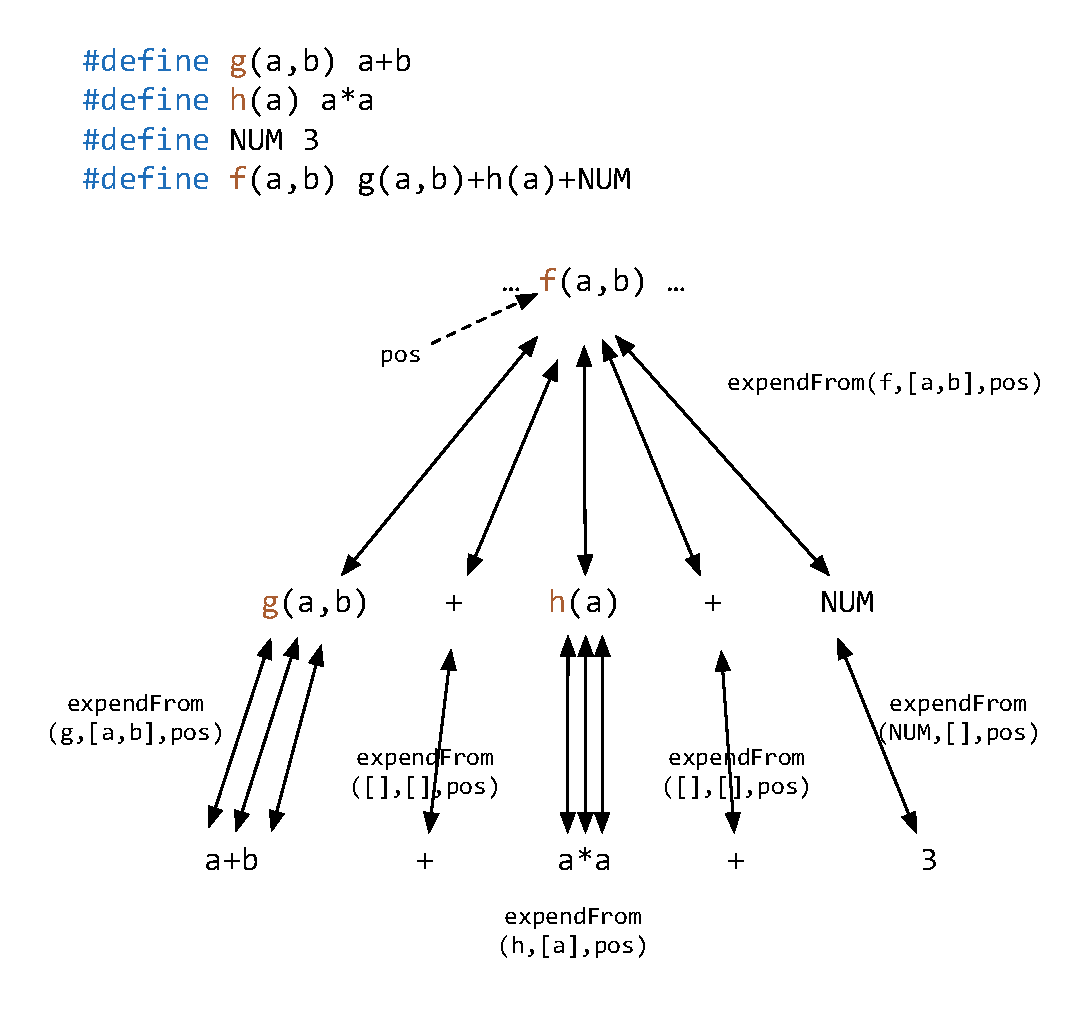
\includegraphics[width=9cm]{pics/original.eps}
\caption{数据结构示例}
\end{figure}
\label{pic:datastruct}
图~\ref{pic:datastruct}展示了宏定义和宏调用展开后的数据结构。构造过程如下:
\begin{itemize}
\item 预处理器扫描源代码发现宏定义指令,将宏定义及其展开式纪录在数据结构中。
\item 当预处理器扫描到位置 $pos$ 时,根据算法规则3,发现函数式宏(\emph{function-like macro})
  调用,分析参数数量,确认宏调用
\item 确认宏调用后,在 $pos$ 位置建立切分点,认为 $f(a, b)$ 是一个独立代码段单元。
  在实现中,这些单元用$Unit$类及其子类实现
\item 独立对$f(a, b)$递归正向展开。正向展开算法在前文中提到(\ref{alg:forward})。
  纪录展开时响应参数位置。
\end{itemize}

图~\ref{pic:datastruct}中的双向箭头表示了词和代码段单元之间的关联关系。
$expandedFrom$中的三个参数表示在下一层的词在正向展开时的来源。
第一个参数描述了该词来源于哪一个宏定义;
第二个参数描述了展开宏时的参数列表,$[]$ 代表空,即没有参数;
第三个参数描述了顶层宏展开在源代码中的位置。
在本例中,第二层中的 $NUM$ 指向第一层的箭头中,$f$ 表示该词被名为 $f$ 的宏展开,
$[a, b]$表示参数列表, $pos$表示展开在源代码中的位置。

我们可以看到,记录下了这些信息和前文提到的重写步骤的信息
可以互换。因此我们就能在这样的数据结构上
应用我们的反向算法,实现双向预处理器。


\subsubsection{BXCPP框架}
我们基于JCPP实现了自己的系统BXCPP。所有的项目代码和试验数据都可以
在我们的项目网站\footnote{\url{https://github.com/harouwu/BXCPP}}上找到。
在此我们简介一下BXCPP框架中主要的几个类。
\begin{figure}
\centering
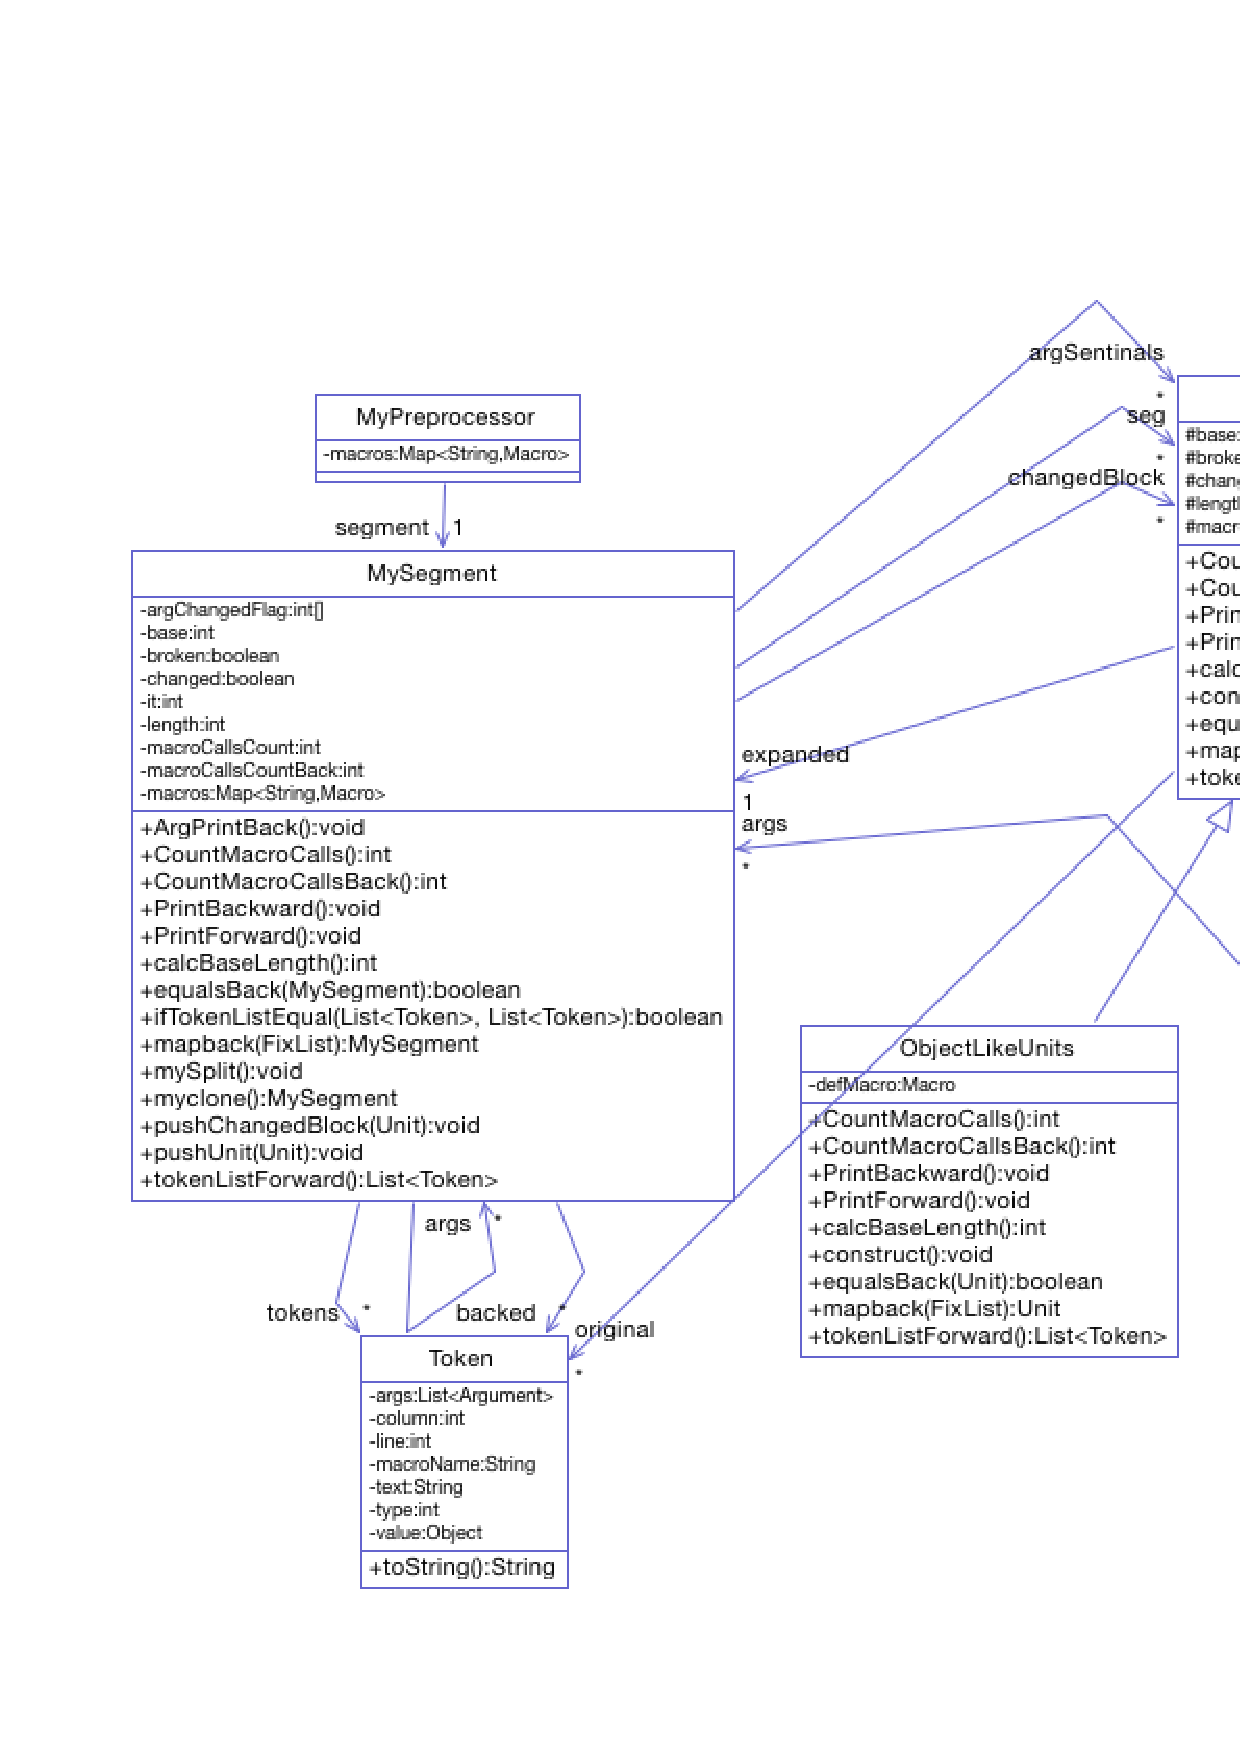
\includegraphics[bb=0 0 1068 746,width=14cm]{pics/class.png}
\caption{主要类类图。}
\end{figure}
\label{pic:classd}

图~\ref{pic:classd}是代码中主要类的类图。小箭头表示包含关系,空心箭头表示继承关系。
我们重写了JCPP中的预处理器 $Preprocessor$类,构造自己的双向C预处理器 $MyPreprocessor$。
该双向预处理器可以识别预处理指令,建立上下文环境纪录和宏定义索引。
同时,双向预处理器把源程序词序列化后,将会把序列保存在类型 $MySegment$里。
$MySegment$封装了词序列和代码段单元序列,同时包含识别拆分代码段单元的函数,类似算法中的$guard$函数。


$Unit$及其子类描述了各种不同类型的代码段单元,他的子类中:
$StringUnit$表示普通文本代码段单元,
$ObjectLikeUnits$表示非函数宏调用代码段单元,
$FunctionLikeUnits$表示函数宏调用代码段单元,
$ArgUnits$表示宏调用参数代码段单元,
$InsertUnit$表示展开式中插入宏参数的代码段单元。

从类图中可以看到,$MySegment$ 和 $Unit$ 类互相包含。
$MySegment$ 中含有 $Unit$ 代码段单元的序列,
而$Unit$在展开时,又包含新的代码段$MySegment$。
这样循环的关系模拟了上一节~\ref{sec:datastruct}中的数据结构,实现了算法。

另外,项目中还定义了许多其他类,如$Token$类描述了词的文本类型等。
具体的项目文档和程序细节,可以访问我们的项目网站了解。
同时我们也实现了前文中提到的 \emph{per-line} 和 \emph{per-file}
两种简单的反向预处理操作。
至此,实现部分基本搭建完成。


\subsubsection{实验基准}
我们的实验在Linux内核版本3.19上执行。我们选择Linux内核源代码因为
Linux是现在最广泛的C语言项目。这之中有许多程序员贡献的代码,包含了不同风格的代码,
也含有大量的预处理指令和宏调用。

为了执行我们的实验,我们需要在Linux内核代码上生成一组修改。
因为我们想看到不同反向预处理算法对程序的影响如何,所以我们需要的修改
应该尽可能出现在有宏调用的函数中。
同时我们在观察中发现,在实际代码中,非函数式宏调用的出现频率
远远高于函数式宏调用。这样导致如果随机生成修改,
大多数修改都会修改非函数式调用,而少数会修改函数式调用。
所以我们根据概率模型,控在非函数式和函数式宏调用的比例为1.5:1。
基于上面的这些计算和宏调用,最终我们从项目中抽取了8000行代码,这之中一共出现了133次宏调用。

接着我们为这抽取的8000行代码生成一组修改。为了模拟现实工程项目中出现的修改,
我们随机性地生成两类修改操作。
第一种是词级别的修改操作,我们随机地替换、删除或插入一个次。
第二种是语句级别的修改,我们随机地删除一句语句、或者从别处随机抽取一句话插入当前位置。
这两种修改的选择是取自现在主流的代码修改工具的方法~\parencite{le2012genprog,QiMLDW14,kim2013automatic}。
其中,GenProg~\parencite{le2012genprog} 和
RSRepair\parencite{QiMLDW14}会直接食用语句级别的修改。
而第一种词级别饿修改则模拟了 PAR~\parencite{kim2013automatic}
中使用的例如替换参数、修改操作符等细微操作。

More concretely, we had a probability $p$ to perform an operation on
each token, where the operation is one of insertion, replacement and
deletion, which had equal probability. The replacement was performed
by randomly mutating some characters in the token. The insertion was
performed by randomly copying a token from somewhere else. Similarly,
we had a probability $q$ to perform an operation on each statement,
where the operation is copy or deletion. The copied statement was
directly obtained from the previous statement. We recognized a
statement by semicolon.

Different tools may have different editing patterns:
a migration tool typically changes many places in a program, whereas a
bug-fixing tool may change a few places to fix a bug. To simulate these two different
densities of changes, we used two different set of probabilities. For
the high-density changes, we set $p=0.33$ and $q=0.1$. For
the low-density changes, we set $p=0.1$ and $q=0.05$.

We generated ten sets of changes, five with high-density and five with
low-density. The number of the changes generated for each set is shown in Table~\ref{tbl:changes}.
\begin{table}[htbp]
\caption{Changes generated for the experiment}\label{tbl:changes}
\centering
% \begin{tabular}{|l|lllll|lllll|}
%   \hline
%   Density & \multicolumn{5}{c|}{Low} & \multicolumn{5}{c|}{High} \\
%   \hline
%   Set & 1 & 2& 3& 4 & 5 & 6 & 7 &8 &9 &10\\
%   \hline
%   Changes & 952 & 885 & 956 & 967 & 884 & 3133 & 3136 & 3088 & 3123 &
%                                                                       3048 \\
% \hline
% \end{tabular}
\begin{tabular}{|l|l|lllll|}
  \hline
  \multirow{2}{2cm}{Low Density} & Set & 1 & 2 & 3 & 4 & 5  \\
  \cline{2-7}
                                 & Changes & 952 & 885 & 956 & 967 & 884 \\
  \hline
  \multirow{2}{2cm}{High Density} & Set & 6 & 7 & 8 & 9 & 10 \\
  \cline{2-7}
                                 & Changes & 3133 & 3136 & 3088 & 3123 & 3048\\
  \hline
\end{tabular}
\end{table}

\subsubsection{Independent variables}
We considered the following independent variables. (1)
\emph{Techniques}, we compared our approach with the two naive
solutions, per-file and per-line. (2) \emph{Density of changes}, we
evaluated both on the five high-density change sets and the five
low-density change sets. % (3) \emph{Types of changes}, we distinguished token-level changes, statement-level changes, and
% combinations of them.

\subsubsection{Dependent variables}
We considered two dependent variables. (1) \emph{Number of remaining
  macro invocations}. We re-ran the preprocessor after the backward
transformation, and counted how macro invocations are expanded during
preprocessing. Since none of the techniques will actively introduce
new macro invocations% \footnote{Strictly speaking, new macro
  % invocations may be introduced passively by the user, e.g., a token
  % is accidentally changed into an object-like macro. Since the
  % probability is very small, we can safely ignore these cases.}
, the
number of expanded invocations is the number of remaining invocations.
To avoid noise from included files, we count only the macro
invocations in the current file.
(2) \emph{Number of errors}. We re-ran the preprocessor, and compared
the new preprocessed program with the previously changed program by
Unix file-comparing tool $fc$. Every time $fc$ reported a difference,
we counted it as an error. (3) \emph{Failures}. Our approach may fail
to propagate the changes, and we record whether a failure is reported
for each change set.

\subsection{Threats to Validity}
A threat to external validity is whether the results on generated
changes can be generalized to real world changes. To alleviate this
threat, we used different types of changes and different density of
changes, in the hope of covering a good variety of real-world changes.

A threat to internal validity is that our implementation of the three
approaches may be wrong. To alleviate this threat, we investigated all
errors we found in the experiments, to make sure it is a true defect
of the respective approach but not a defect in our implementation.

\subsection{Results}
\begin{table}[htbp]
  \caption{Experimental Results}\label{tbl:results}
\centering
\begin{tabular}{|l|l|lllll|}
  \hline
  Low Density & Set & 1 & 2 & 3 & 4 & 5\\
  \hline
  \multirow{3}{*}{Our Approach} &  Macros & 73 & 75 & 72 & 80 & 81 \\
  \cline{2-7}
              &Errors & 0 & 0 & 0 & 0 & 0  \\
  \cline{2-7}
              & Failures & n & n & n & n & n \\
  \hline
  \multirow{3}{*}{Per-Line} & Macros & 23 & 25 & 23 & 20 & 26 \\
  \cline{2-7}
              & Errors & 6 & 7 & 6 & 7 & 7  \\
  \hline
  \multirow{3}{*}{Per-File} & Macros & 0 & 0 & 0 & 0 & 0  \\
  \cline{2-7}
              & Errors & 0 & 0 & 0 & 0 & 0 \\
  \hline
  \hline
  High Density & Set & 6 & 7 & 8& 9& 10\\
  \hline
  \multirow{3}{*}{Our Approach} &Macros & 47 & 51 & 53 & 48 & 44 \\
  \cline{2-7}
              &  Errors & 0 & 0 & 0 & 0 & 0  \\
  \cline{2-7}
              & Failures & n & n & n & n & n \\
  \hline
  \multirow{3}{*}{Per-Line} & Macros & 9 & 7 & 7 & 8 & 10  \\
  \cline{2-7}
              & Errors & 6 & 6 & 7 & 6 & 6 \\
  \hline
  \multirow{3}{*}{Per-File} & Macros & 0 & 0 & 0 & 0 & 0  \\
  \cline{2-7}
              & Errors & 0 & 0 & 0 & 0 & 0 \\
  \hline\end{tabular}
\\
\parbox{\columnwidth}{\footnotesize Row ``Macros'' shows the number of
    remaining macros. Row ``Errors'' shows the number of errors caused. Row ``Failures'' indicates whether a
    failure is reported in the backward transformation.}
\end{table}
% \begin{table*}[htbp]
% \caption{Macros remainings and errors of different algorithms and data set}
% \centering
% \begin{tabular}{l|cc|cc|cc}
% \hline
% Algorithm  &High Mutation & &Low Mutation & &Average &  \\
%  &Remain &Error &Remain &Error &Remain &Error \\
% \hline
% CPP-TRANS &120 &0 &243.8 &0 &181.9 &0 \\
% PER-FILE &0 &0 &0 &0 &0 &0  \\
% PER-LINE &25.6 &5.8 &64.2 &2.4 &44.9 &4.1 \\
% \hline
% \end{tabular}
% \end{table*}

The result of our evaluation is shown in Table~\ref{tbl:results}. We
discuss the results with respect to the research questions below.

\subsubsection{RQ1} As we can see, our approach preserves macro invocations. Per-line preserves very few macro
invocations, while per-file, as we expected, preserves no macro
invocations. We further investigated why per-line preserves so few
macro invocations. One main reason we found is that there are usually
multiple macro invocations per line, and per-line will expand all of
them if any tokens in this line is changed.
\subsubsection{RQ2} Our approach and per-file lead to no errors while
several errors are caused by per-line. This is because there are quite
a few macro invocations that cross multiple lines. These macros 
take expressions or statements as argument, which are usually too long
to be included in one line.
\subsubsection{RQ3} As discussed before, our approach may report a failure during the
backward transformation. This is usually because the changes
accidentally introduce a new macro invocation in the preprocessed code, where there is no way
to satisfy PUTGET. 
However, we do not
observe any such cases in our experiment. The reason is that
macros usually have special names and it is not easy to collide with a
macro name by copying or mutation. Note the other two
approaches never report a failure, so the corresponding fields in Table~\ref{tbl:results} are left blank. 

Although probably being rare in practice, theoretically our approach
may report false alarms: our approach reports a failure but
a correct change on the source program exists. {For example, let consider the
  following code piece,
\begin{lstlisting}
#define p (x)
plus p
\end{lstlisting}
where $plus$ is the macro defined in code
piece~\eqref{eqn:expansion}. After preprocessing, this code piece becomes
$plus\ (x)$. If we change the last parenthesis into $)\ hello$, our
approach reports a failure because first $p$ will be expanded and then
the expanded content forms a new macro invocation with $plus$.
However, there exists a feasible change: replacing $p$ with $hello\ p$.}

%%% Local Variables:
%%% mode: latex
%%% TeX-master: "main"
%%% End:
